\documentclass[paper=a4, fontsize=12pt]{scrartcl} % A4 paper and 11pt font size

% \usepackage[T1]{fontenc} % use 8-bit encoding that has 256 glyphs
\usepackage{fourier}     % use the Adobe Utopia font for the document
                         % (comment this line to return to the LaTeX default)
%\usepackage{babel} % English language/hyphenation
\usepackage{amsmath,amsfonts,amsthm} % math packages
\usepackage{subeqnarray}

\usepackage{lipsum} % used for inserting dummy 'Lorem ipsum' text into the template
\usepackage{bold-extra}

\usepackage{gensymb}
\usepackage{listings}
\usepackage[utf8]{inputenc}
\usepackage{centernot}
\usepackage{mathrsfs}
\usepackage{amssymb}
\usepackage{physics}
\usepackage{verbatim}
\usepackage{fancyvrb}
\usepackage{biblatex}

% default fixed font does not support bold face
% \DeclareFixedFont{\ttb}{T1}{txtt}{bx}{n}{12} % for bold
% \DeclareFixedFont{\ttm}{T1}{txtt}{m}{n}{12}  % for normal

% custom colors
\usepackage{color}
\definecolor{deepblue}{rgb}{0,0,0.5}
\definecolor{deepred}{rgb}{0.6,0,0}
\definecolor{deepgreen}{rgb}{0,0.5,0}
\definecolor{lightblue}{rgb}{0.95,0.95,1}
\definecolor{lightgrey}{rgb}{0.6,0.6,0.6}
\usepackage{listings}

% use graphics packages
\usepackage{graphicx}
\usepackage{float}
\usepackage{tikz}
\usetikzlibrary{matrix}
\usetikzlibrary{calc}
\usetikzlibrary{patterns,fadings}

% python style for highlighting
\newcommand\pythonstyle{\lstset{
language=Python,
backgroundcolor=\color{lightblue},
basicstyle=\ttm,
otherkeywords={self,def},             % add keywords here
keywordstyle=\ttb\color{deepblue},
emph={while,for,if,elif,else,def,as,shape,conj,dot,copy,flatten,eye,zeros,ones,hstack,vstack,real,imag,conjugate,sin,cos,exp,append,insert,index,__main__}, % custom highlighting
%emphstyle=\ttb\color{deepred},     % custom highlighting style
emphstyle=\ttb\color{deepblue},     % custom highlighting style
stringstyle=\color{deepgreen},
commentstyle=\color{lightgrey},
frame=tb,                         % any extra options here
numbers=left,
showstringspaces=false            %
}}

% python environment
\lstnewenvironment{python}[1][]
{
\pythonstyle
\lstset{#1}
}
{}

% python for external files
\newcommand\pythonexternal[2][]{{
\pythonstyle
\lstinputlisting[#1]{#2}}}

% python for inline
\newcommand\pythoninline[1]{{\pythonstyle\lstinline!#1!}}


\usepackage{sectsty}        % allows customizing section commands
\allsectionsfont{\normalfont\scshape}      % make all sections centered
                                                      % the default font and small caps
\newcommand{\ssubsection}[1]{%
  \subsection[#1]{\raggedright\normalfont\itshape #1}}

\usepackage{fancyhdr}        % custom headers and footers
\pagestyle{fancyplain}       % makes all pages in the document conform to
                             % the custom headers and footers

% \renewcommand{\sectionmark}[1]{\markright{\thesection\ #1}}
\renewcommand{\sectionmark}[1]{\markboth{\thesection\ #1}{}}
\fancyhead[L]{\footnotesize\scshape\leftmark}
\fancyhead[R]{Page \thepage}


                             % the same way as the footers below
\fancyfoot[L]{\textit{Christopher R. McLeod}}              % empty left footer
\fancyfoot[C]{}              % empty center footer
\fancyfoot[R]{\textit{00947553}}      % page numbering for right footer
\renewcommand{\headrulewidth}{0.5pt}     % add header underlines
\renewcommand{\footrulewidth}{0.5pt}     % add footer underlines
\setlength{\headheight}{13.6pt}        % customize the height of the header



\numberwithin{equation}{section}       % number equations within sections
                                       % (i.e. 1.1, 1.2, 2.1, 2.2 instead of 1, 2, 3, 4)
\numberwithin{figure}{section}         % number figures within sections
                                       % (i.e. 1.1, 1.2, 2.1, 2.2 instead of 1, 2, 3, 4)
\numberwithin{table}{section}          % number tables within sections
                                       % (i.e. 1.1, 1.2, 2.1, 2.2 instead of 1, 2, 3, 4)

\setlength\parindent{24pt}         % removes all indentation from paragraphs
                                  % comment this line for an assignment with lots of text


% \usepackage[T1]{fontenc}
\usepackage{enumerate}

% \usepackage[tocflat]{tocstyle}
\allowdisplaybreaks
\makeatletter
\setcounter{tocdepth}{4}
% \renewcommand\tableofcontents{%
%   \null\hfill\textsc{\Large\contentsname}\hfill\null\par
%   \vspace{1cm}
%   \@mkboth{\MakeUppercase\contentsname}{\MakeUppercase\contentsname}%
%   \@starttoc{toc}%
% }
% \renewcommand*\l@section{\ifnum\c@tocdepth>\z@\vskip 6pt plus 1pt minus 1pt \fi
%                          \@dottedtocline{1}{1.5em}{2.3em}}
% \renewcommand{\@pnumwidth}{1.75em}
% \renewcommand{\@tocrmarg}{2.75em}
\makeatother
\usepackage{empheq}


%--------------------------
%	TITLE SECTION
%--------------------------
\renewcommand*\contentsname{Summary}

\newcommand{\horrule}[1]{\rule{\linewidth}{#1}} % create horizontal rule command
                                                % with 1 argument of height


\renewcommand*\footnoterule{}


\title{
\normalfont \normalsize
\textsc{Imperial College London, Department of Mathematics} \\ [25pt]
\horrule{0.5pt} \\[0.4cm]                      % thin top horizontal rule
\huge M4N9 Project 3: \\ Exploiting Matrix Structure in Iterative Algorithms \\           % the assignment title
\horrule{2pt} \\[0.5cm]                        % thick bottom horizontal rule
}


\author{Christopher McLeod}
\date{\normalsize\ January 12, 2018}

\begin{document}
%\ttfamily
%\fontseries{b}\selectfont

\titlepage
\maketitle
\begin{center}
  
\includegraphics[width=100pt]{crest.png} \\

\end{center}
\thispagestyle{empty}

%-----------------------------------------------------------------------
% contents page
%-----------------------------------------------------------------------
\newpage
\thispagestyle{empty}
\tableofcontents
\newpage

%-----------------------------------------------------------------------
% Rest of Paper
%-----------------------------------------------------------------------

\section*{\centerline{Foreword}}

In the interest of making this paper as concise as possible, in general functions and scripts have been excluded from the final write-up. What is included is a description of the algorithms and programs, in terms of what function they perform. For the implementation,the code is provided alongside this paper with detailed comments.\\

\section{part 1}
\subsection{One}
Since $P$ is a permutation matrix, $P^TP = I$ and so $L = P^T (-D + V_{N}) P$ is a similarity transformation of ${-D + V_N}$. From lectures we saw that similar matrices have identical eigenvalues. This means that if we solve for the eigenvalues of $L$, the pentadiagonal matrix, then we have solved exactly for the eigenvalues of $[-D + V_N]$

\subsection{Two}
The function \texttt{tridiagonalize} takes a pentadiagonal matrix and transforms it via Givens rotations to a tridiagonal matrix. The algorithm implements the method from the Schwarz journal \cite{1} in which givens rotations are used to help transform the symmetric pentadiagonal matrix $L$ into the symmetric tridiagonal matrix $T$. Of course because the method successively left-multiplies $L$ with the transpose some Givens matrix $G^T$ and then immediately right-multiplies $L$ by G, $T$ is similar to $L$ ($G^TG = I$) and so solving for the eigenvalues of $T$ is to solve exactly for the eigenvalues of $L$. \\
\indent In the first step of the \texttt{tridiagonalize} function, the terms one and two below the main diagonal entry $L_1,1$ are selected to be $'a'$ and $'b'$ respectively. The function \texttt{givens} then rotates it to a point $(r,0)$ in the $a-b-$plane. It does this by finding the values $c = \cos(\theta)$ and $s = \sin(\theta)$ such that 
$$
\begin{bmatrix}
c & s \\
-s & c \\ 
\end{bmatrix} ^ T
\begin{bmatrix}
a \\
b \\ 
\end{bmatrix}
= 
\begin{bmatrix}
r \\
0 \\ 
\end{bmatrix}
$$
where $r = \sqrt{a^2 + b^2}$. This can be easily be solved explicitly for the cases $\abs{a} > \abs{b}$ or $\abs{a} \leq \abs{b}$, assuming b is non-zero. \\
Hence left multiplying by the Givens matrix $G(2,3,\theta)^T$ turns the second entry below the $1^{st}$ main diagonal term to 0. By symmetry, multiplying $L$ by $G(2,3,\theta)$ on the right also clears out the second term on the right of the $1^{st}$ main diagonal term, i.e. $[G(2,3,\theta)^TLG(2,3,\theta)]_{1,2} = [G(2,3,\theta)^TLG(2,3,\theta)]_{2,1} = 0$. Consequently, however there now appears two pesky terms outside of the band! These terms are identical and occur in symmetric positions outside of the band in positions $(1,4)$ and $(4,1)$.\\
\cite{1}  details a way in which these terms can be eliminated by using further Givens rotations (and hence preserving the similarity of $T$ and $L$). By similarity, we need only consider the elements above the main diagonal. W.r.t fig 1.1, we carry out the plane rotation on the 'out-of-band' term and the band-element to its left. This 'pushes' it down by left multiplying by a suitable $G(3,4,\phi_1)^T$, then right multiplying $G(3,4,\phi_1)$. This produces an element $'g'$ in the third row and seventh column, which is in turn eliminated similarly by $G(6,7,\phi_2)$ for appropriate $\phi_2$.

\begin{center}
	\begin{figure}[h!]
	  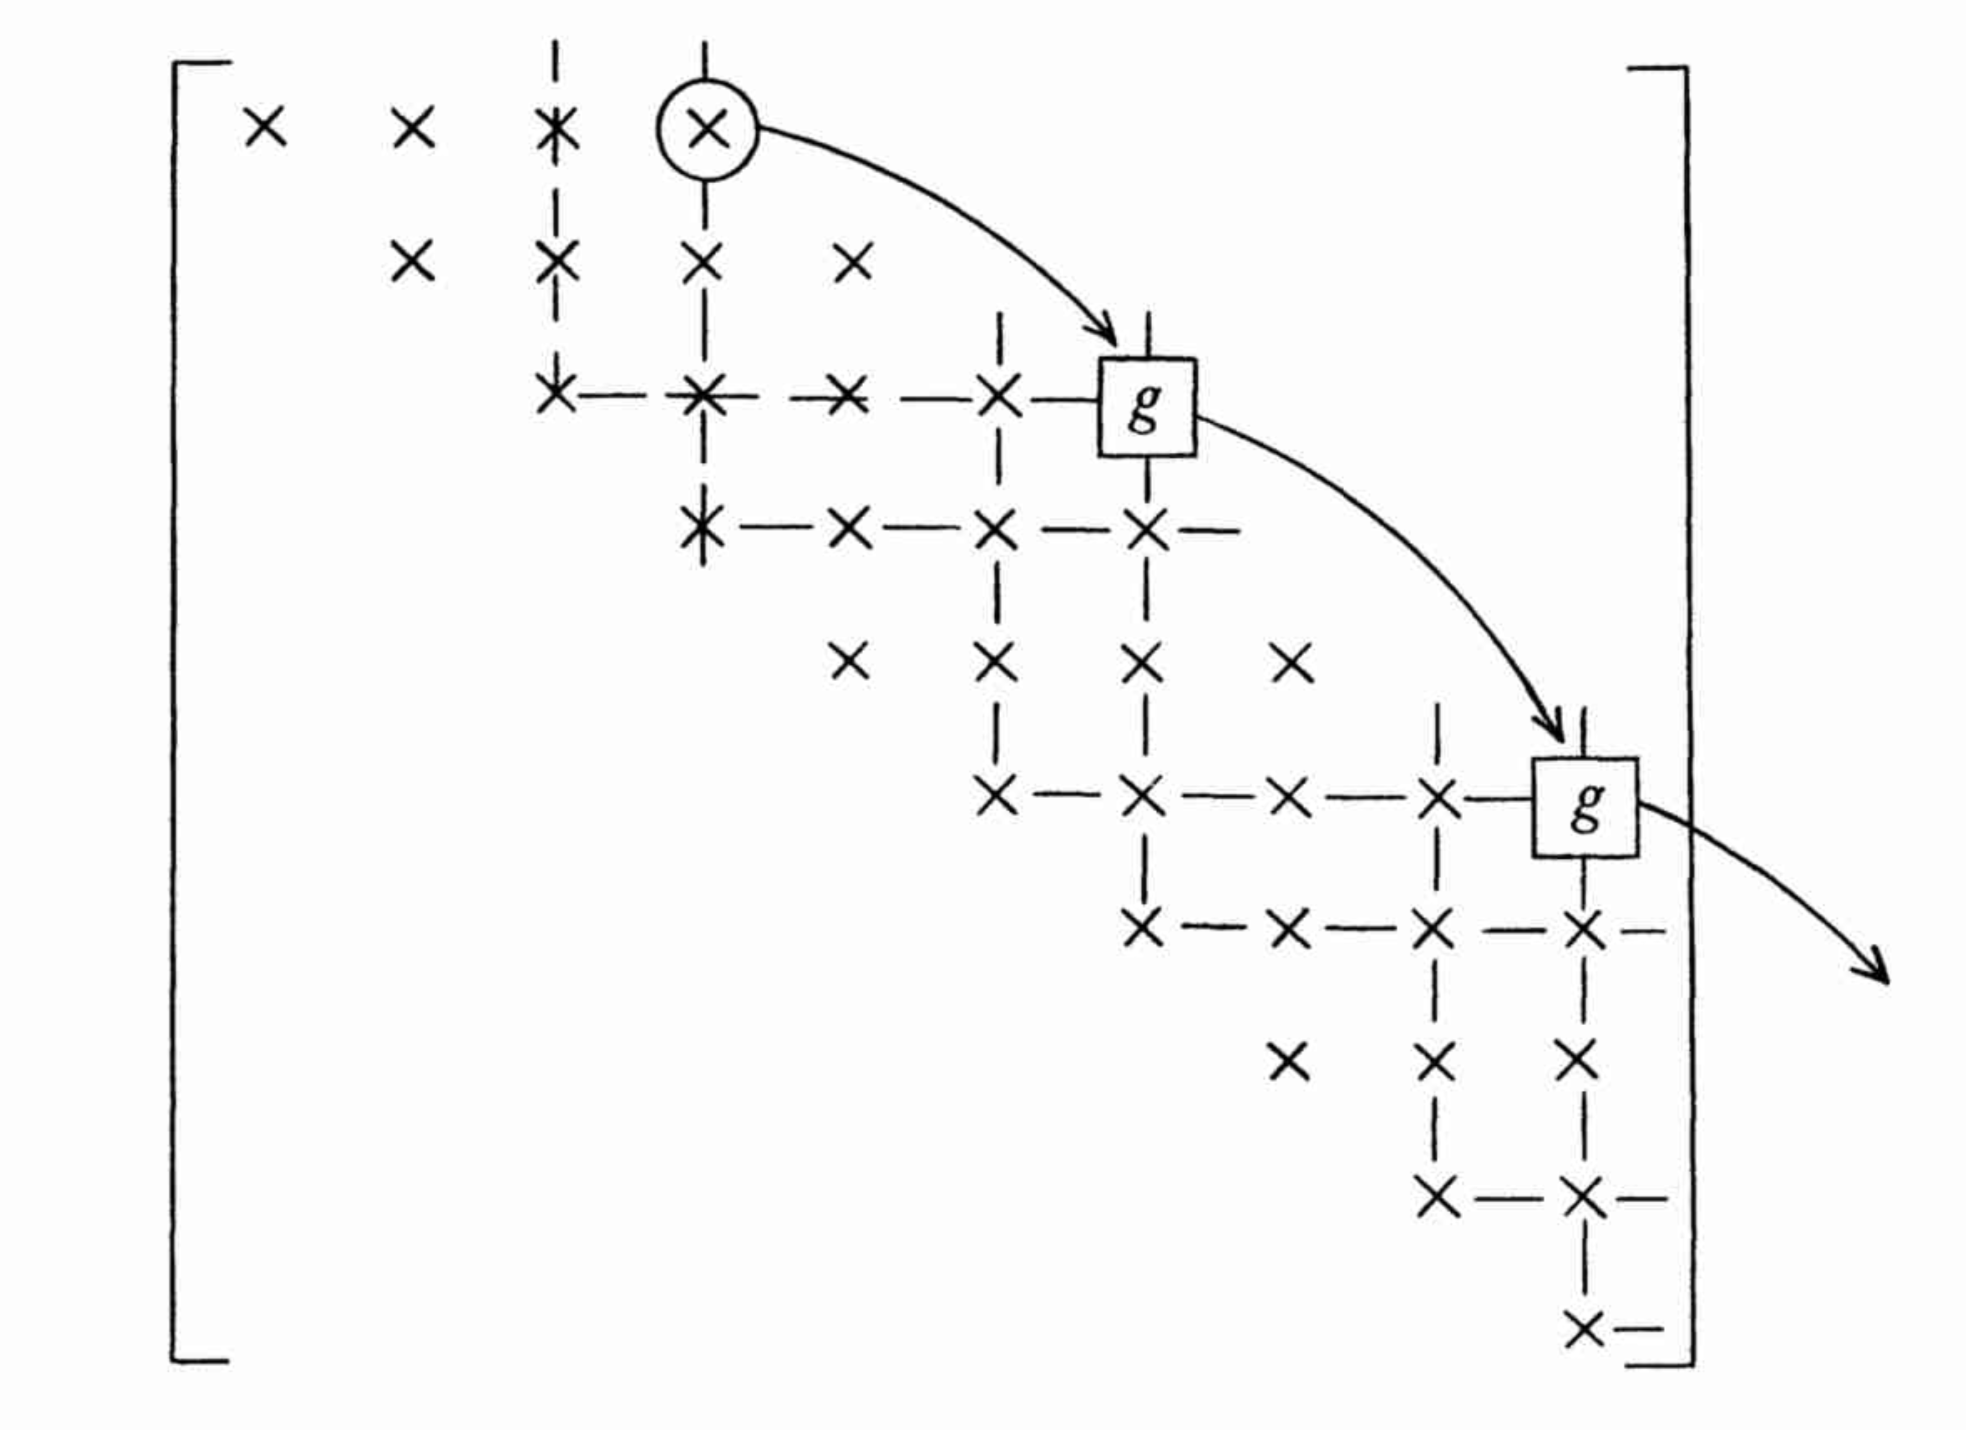
\includegraphics[width=\linewidth]{outofband}
	  \caption{\cite{1}:Givens Rotations push the out-of-band term out}
	  \label{fig:outofband}
	\end{figure}
\end{center}


\noindent These rotations are continued until the out-of-band term has been pushed outside the matrix dimensions. \\
As described, the above is a repeatable process. The steps are to eliminate the $2^{nd}$ subdiagonal terms and chase out the out-of-band terms. The terms need to be chased out so long as $\lfloor (N - j - 2)/2 \rfloor >0$ where $j$ is the step number of the algorithm and N is the length of the (square) matrix. \\
\\
The described method is implemented in \texttt{tridiagonalize} but certain speed-ups are used by taking advantage of matrix structure. For example, we only multiply the $2\times 5$ sub-matrix of $L$ (or its updated value if $j > 1$) which is actually affected by the Givens matrix by the $2\times 2$ matrix $[c s; -s c]$ (the non-identity part of the Givens matrix). This reduces the $O(N^2)$ matrix multiplication task to an $O(1)$ one. Note, The 5 appears as to make sure the multiplication captures the terms within the band-with.\\
\\
Whereas Householder-based methods from class require $O(N^3)$ FLOPs, the Givens procedure requires only $O(N^2)$ in total. \\
\indent To see this, consider the code of \texttt{tridiagonalize}. In the first for loop, we carry out 1 Givens rotation, which requires 5 FLOPs. Next 2 matrix multiplications of size $leq 30$ (calculated using matrix multiplication of $2\times 5$ and $2\times 2$). In the second for loop we carry out two more matrix multiplications of the same size. In total, the worst case scenario equates to

$$
(N-2)[65 + \sum_{j=1}^{\lfloor N - j - 2 \rfloor} 60] \approx O(N^2) 
$$

\noindent FLOPs. To demonstrate this, a log-log plot of run-time of the \texttt{tridiagonalize} algorithm for different N via \texttt{tridiagTime} is shown in fig \ref{fig:log-log_tridiag}. N is allowed to take on values 400, 800, 1200, 1600, 2000, 2400, 2800, 3200 and the resulting pentadiagonal matrix of length N is created using the Schrodinger script (turned function) The result of a linear regression of the log-run-times against the log-N values gives \texttt{grad = 1.9587}. This is pretty good evidence to support the claim that the procedure executes in $O(N^2)$ time. 


\begin{center}
	\begin{figure}[h!]
	  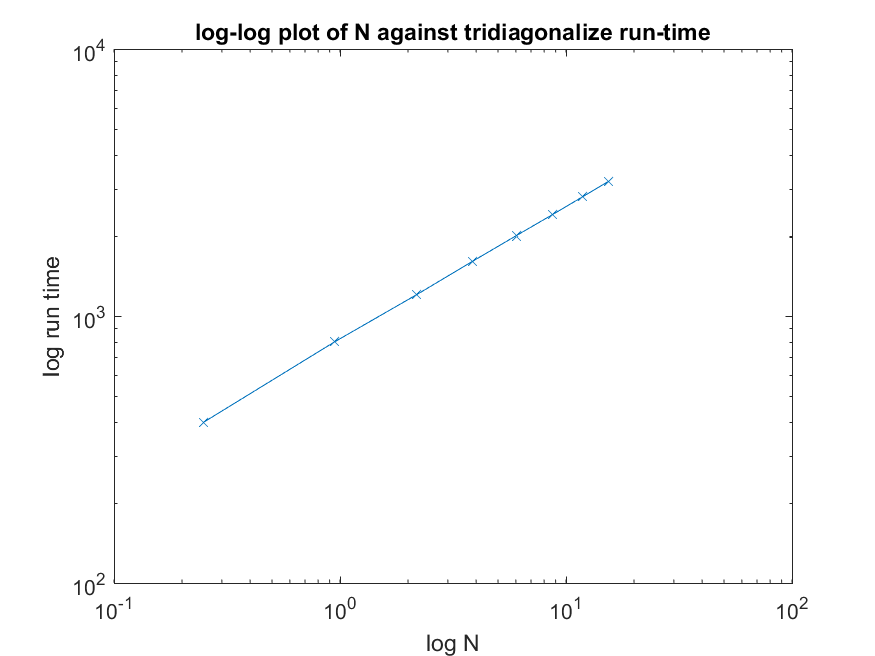
\includegraphics[width=\linewidth]{log-log_tridiag}
	  \caption{run-time of \texttt{tridiagonalize} against N}
	  \label{fig:log-log_tridiag}
	\end{figure}
\end{center}


\subsection{Three}
\texttt{wilkinsonQR} is the function which computes the eigenvalues of the input matrix $T$ via the $QR$ algorithm with Wilkinson-shift. The Wilkinson-shift is chosen as it is guaranteed to converge globally and does so in at worst quadratic time when the algorithm includes deflation\cite{2}. \\ 
\indent The algorithm calculates the Wilkinson-shift $\mu$, then $T = T - \mu I$, then the QR-decomposition of this updated $T$. From here, $RQ$ is calculated, and we restore $T = QR + \mu I$, as per the usual shifted-QR algorithm. As a speed up, it also deflates. This means that for $T$, the entry $T_{N, N-1}$ shrinks to near 0 and the algorithm is recursively applied to $T(1:N-1, 1:N-1)$. This means that the QR iteration converges globally and quadratically. \\
\indent Instead of explicitly calculating $Q$ and $R$ and multiplying, $R$ decomposition is via the function \texttt{RP}) and storing the $\cos$ and $\sin$ values of the Givens rotations required to create it. The $RQ$ step of the $QR$-algorithm is done implicitly. This is faster, as instead of multiplying two $N\times N$ matrices, we compute $N-1$ multiplications of a $N \times 2$ matrix and a $2\times 2$ ($O(N^3)$ vs $O(N^2)$). \texttt{RP} itself requires $(N-1)[5 + 12] \approx O(N)$ FLOPs (5 FLOPs for the Givens function and 12 for the multiplication of two $2\times 2$ matrices). So in total, the $T = QR$ and $T = RQ$ steps can be done in just $O(N^2)$ flops instead of $O(N^3)$. \\
To give evidence to this, \texttt{wilkinsonAnalysis} run with the 'timer' flag set to true returns the log-log plot \ref{fig:log-log_wilkinson} of run-time against N. 

\begin{center}
	\begin{figure}[h!]
	  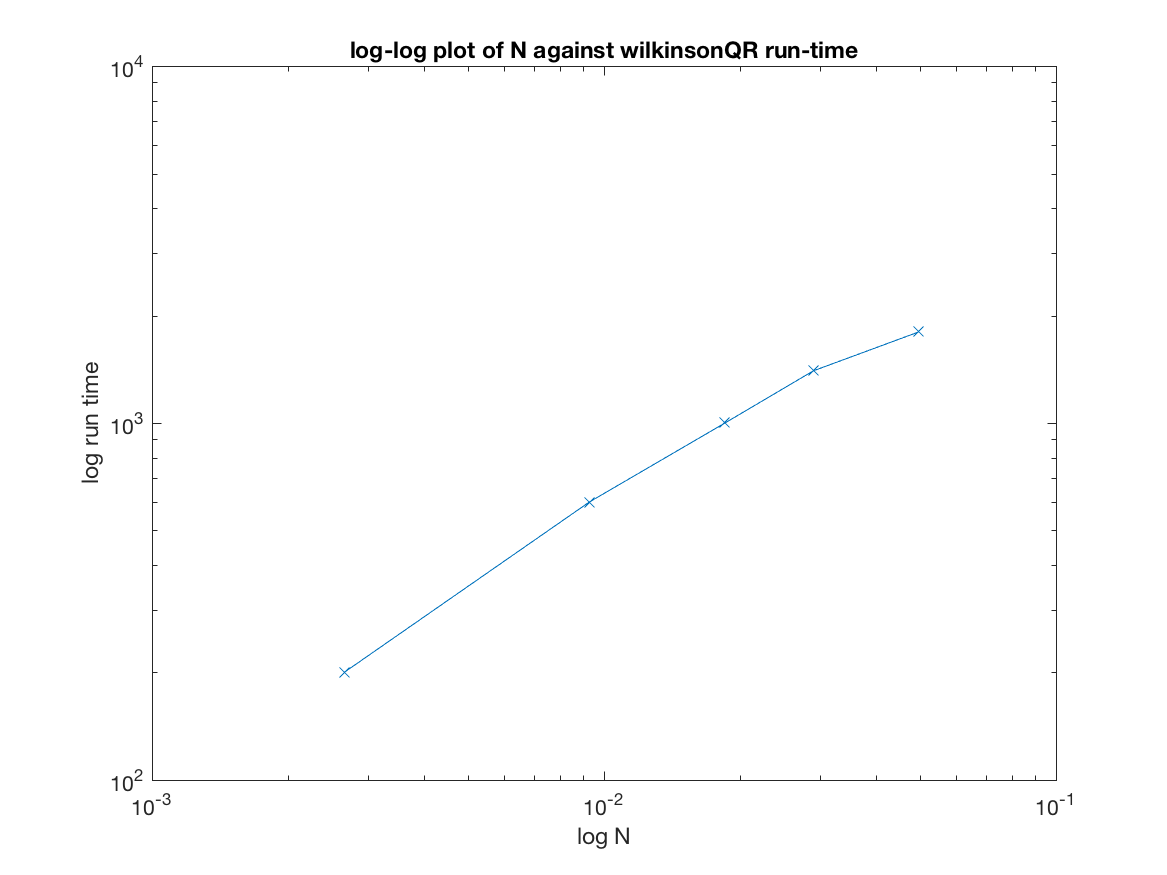
\includegraphics[width=\linewidth]{log-log_wilkinson}
	  \caption{run-time of QR and implicit RQ in \texttt{WilkinsonQR} against N}
	  \label{fig:log-log_wilkinson}
	\end{figure}
\end{center}

\noindent with a linear regression returning the gradient of \texttt{grad = 1.2973}. This is smaller than expected. This is due to the sparse nature of $R$ and matlab's ability to multiply sparse matrices quickly, meaning that the implicit multiplication $RQ$ actually takes less than $O(N^2)$ in practice. \\

\texttt{wilkinsonAnalysis} also creates a plot for the ascending sorted energy levels (i.e. the eigenvalues of $T$) $E_n$ against their index, when the flag \texttt{evalplot} is set to be true. This can be seen in fig \ref{fig:evalplot}. \\

\begin{center}
	\begin{figure}[h!]
	  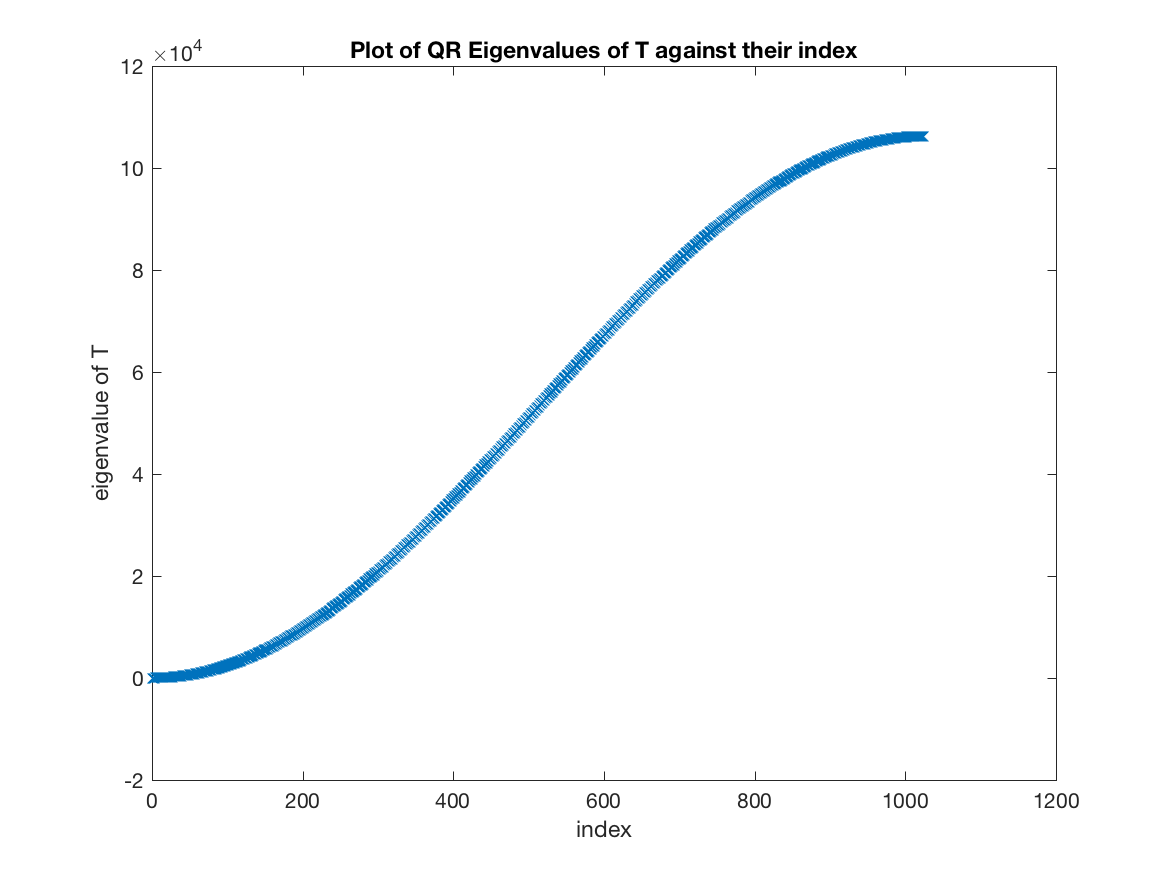
\includegraphics[width=\linewidth]{evalplot}
	  \caption{plot of sorted eigenvalues against their index}
	  \label{fig:evalplot}
	\end{figure}
\end{center}

If the final flag \texttt{lowtable} is set true, the function also produces a table of the lowest ten energy levels. The result is visible in \ref{table:1}
\begin{table}
	\begin{center}
		\begin{tabular}{c}
		     $E_n$ \\ 
			\hline 
		
		    -159.06 \\
		    -85.625 \\
		    -30.858 \\
		    -1.2203\\
		    0.32089\\
		     2.1454\\
		      2.869\\
		     7.1873\\
		     7.8826\\
		      14.69\\
		
		\end{tabular}
	\end{center}
	\caption{10 lowest energy levels $E_n$}
	\label{table:1}
\end{table}

I don't believe it is worth trigularizing the pentadiagonal matrix for the sake of the QR. Doing so allows for a very quick QR, RQ step in \texttt{wilkinsonQR} but, to do the same thing with a pentadiagonal matrix takes twice as long. Comparing this with the $O(N^2)$ that is needed to triagularize the matrix, it does not seem to benefit the number of FLOPs required significantly. 

\newpage

\subsection{Four}
Using the eigenvalues computed from the \texttt{wilkinsonQR}, the function \texttt{invItr} computes the wave functions $\Psi_n$ (i.e. the eigenvectors of T)  that have negative energy, as well as the one corresponding to the 100th positive eigenvalue. \\
\indent \texttt{invItr} performs the inverse iteration algorithm using the known eigenvalues from \textbf{Three} (after selecting them from the lot to be the above eigenvalues).\\
\indent The algorithm has been adapted for matrix structure. Since the condition number of $T - \lambda_j I$ is extremely high for many eigenvalues $\lambda$, it is not possible to exploit the tridiagonal structure of $T$ in the step of the algorithm which involves solving the system $(T - \lambda I)w = v$. Instead, we settle for solving the pentadiagonal system $(L - \lambda I)w = v$ at every iteration. Since computing the QR decomposition of the pentadiagonal system involves one more lot of givens rotations (whch are O(1)), this takes about twice as long as solving the tridiagonal system, but still requires only $O(N)$ computations. \\
\texttt{pentDiagSove} solves Lw = v for w. performing N -2 Givens rotations on the second off diagonal below the main of L (acting on the first subdiagonal). It left multiplies $[c s; -s c]^T$  with the relevant part of R (a $2\times 5$ sub matrix) and the relevant two entries of v. It does this again for the first subdiagonal below the main diagonal (acting on the main diagonal). These are done in $O(N)$ FLOPs each. Lastly it carries out a backward substitution which is tailored for the banded system. \texttt{bandBacksub} uses the bandwidth of $L$ to reduce the number of computations to only those necessary for back substitution. As opposed to the regular backsub which requires $O(N^2)$, \texttt{bandBacksub} requires only $2qN \approx O(N)$ FLOPs, where q is the bandwidth of $L$ (5 in this case).\\
Overall, the pentadiagonal system is accurately solved in $O(N)$ FLOPs. \\
\\
\texttt{psiplot} plots $\abs{\Psi_n}^2$ for the wave-functions of negative energy, as well as for one of positive energy. The results of the plots for the wave-functions of negative energy are presented in \ref{fig:negE} and the plot of the wave function for positive energy is presented in \ref{fig:posE}. 

\begin{center}
	\begin{figure}[h!]
	  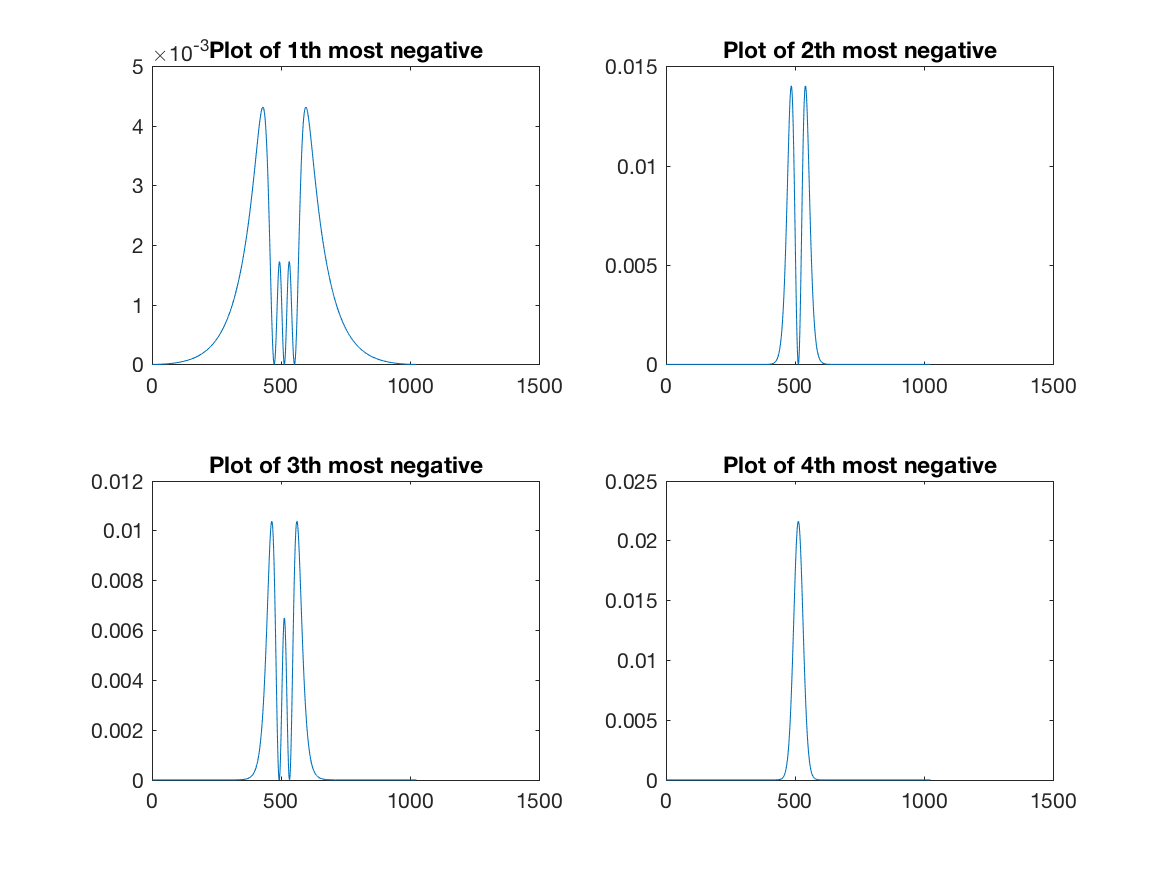
\includegraphics[width=\linewidth]{negPsi}
	  \caption{Plots of $\abs{\Psi_n}^2$ for negative $E_n$}
	  \label{fig:negE}
	\end{figure}
\end{center}


\begin{center}
	\begin{figure}[h!]
	  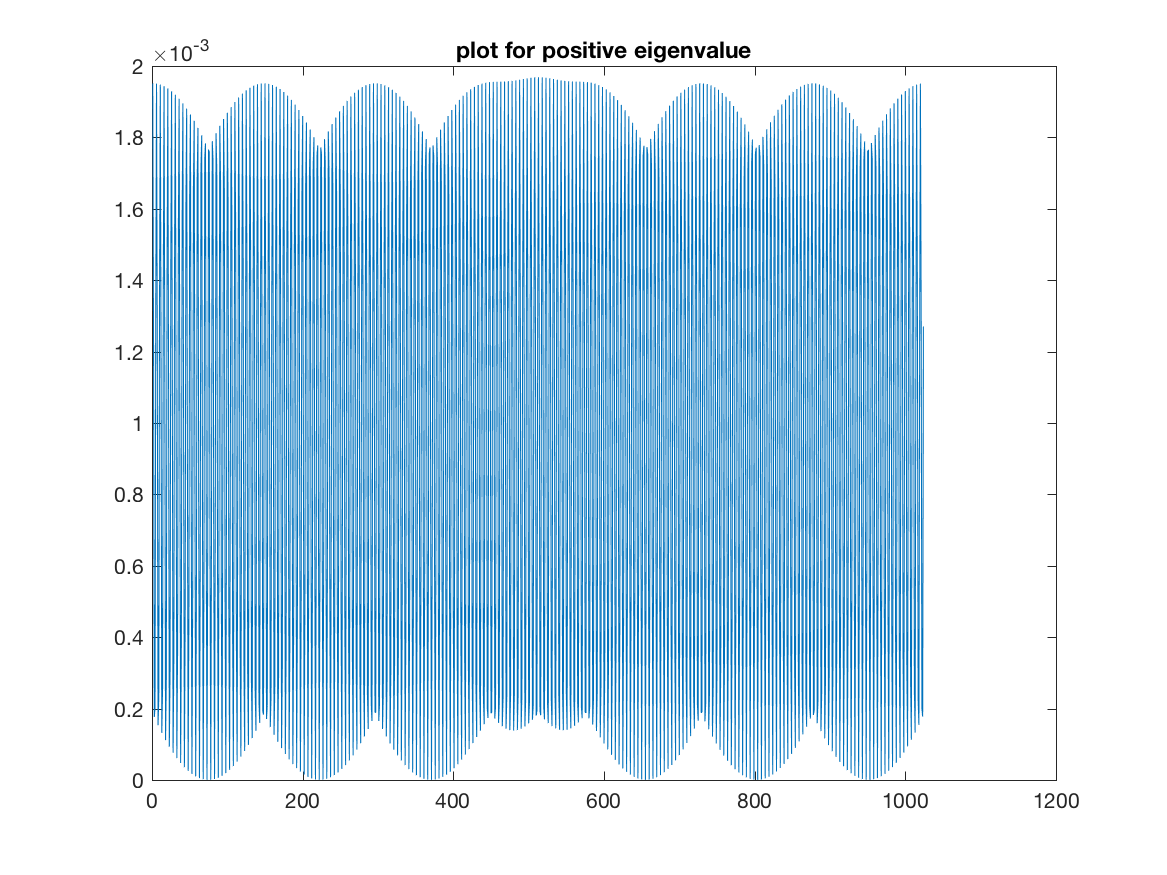
\includegraphics[width=\linewidth]{posPsi}
	  \caption{Plot of $\abs{\Psi_n}^2$ for a positive $E_n$}
	  \label{fig:posE}
	\end{figure}
\end{center}

\noindent Positive energies give wave functions which oscillate very quickly. Wave functions corresponding to negative energies give few well defined peaks. As the magnitude of the energies decreases, the value becomes higher and the number of peaks reduces. 

\newpage

\section{part 2}

\subsection{One} 
The \texttt{LDLt} function computes the $LDL^T$ decomposition of a matrix, should it have one. We choose $LDL^T$ as for symmetric positive definite matrices the $LDL^T$ decomposition is guaranteed to exist and can be found in approximately half the time it would take to obtain its Cholesky decomposition. The system is also solved in $O(N^2)$ which is approximately the same as the Cholesky system. M is dense which means without preconditioning, we wont find a quicker factorisation. \\
\texttt{qu1} varies $\gamma$ from 0.1 to 0.9 in steps of 0.1 and creates the portfolio for the different $gamma$ and returns the table \ref{table:2}

\begin{table}
	\begin{center}
		\begin{tabular}{c |c | c || c | c}
	
$\gamma$  & ret     &     risk  &         $x^{\star}_{max}(1)$ & $x^{\star}_{max}(2)$ \\
	\hline

 0.1 &    0.003971  &   0.0016485&          1&    2.757e-07\\
 0.2 &   0.0038952  &   0.0012048&    0.68542   &   0.31458\\
 0.3 &    0.0038596  &   0.0010933 &   0.54177    &  0.45298\\
 0.4 &    0.0037326  &  0.00085516  &  0.39333     &   0.375\\
 0.5 &    0.0036309  &   0.0007283   & 0.33712      & 0.29798\\
 0.6 &   0.0035597  &  0.00066937 &   0.36699      & 0.29869\\
 0.7 &   0.0034729  &  0.00062236 &   0.38673      & 0.26492\\
 0.8 &    0.003372  &  0.00058813 &   0.38001&      0.23329\\
 0.9 &   0.0023149  &  0.00042129 &    0.2823 &     0.10539\\

		
		\end{tabular}
	\end{center}
	\caption{Risk return portfolio for varying $\gamma$ }
	\label{table:2}
\end{table}




\subsection{Two}
If we create the symmetric tridiagonal matrix Z such that 
$$
Z_{ij} = 
\begin{cases}
	1 &\text{if $j=i$ for i,j < N}\\
	-1& \text{if $j = i + 1$}\\
	0 & \text{o/w}
\end{cases}
$$

\noindent i.e 
$$
Z = 
\begin{bmatrix}
     1 & -1 & 0  &\cdots & \, & 0 & 0 \\
     -1 & 1  & 0 &\cdots & \, & 0& 0 \\
     0 & -1 & 1 & \cdots & \, & 0& 0 \\
	\vdots & \vdots & \, & \ddots & \,  & \vdots & \vdots \\
	0 & 0 & 0 &   \cdots& &  1 & 0 \\
	0 & 0 & 0  & \cdots & \, & 0 & 0
\end{bmatrix}
$$

\noindent Then for any column $v$ of $Z$ we have either 
$$ v = 
\begin{bmatrix}
\boldsymbol{0} \\
-1 \\
1 
\end{bmatrix}, \; 
\text{or}
v = \boldsymbol{0}
$$

\noindent In any case, $\sum_{j=1}^{N} v_{j} = [ \mathbb{1}^T Z ]_j = \boldsymbol{0}$.

\subsection{Three} 
Note letting

\begin{align*}
\tilde{M} &= Z^T M Z \\
&= Z^T (2\Sigma + \Phi(x_n)) Z \\
&= 2Z^\Sigma + Z^T \Phi Z \\
\end{align*}
Means that for any vector $x$ we let $y = Zx$ then we get 
$$
x^T \tilde{M} x = 2y\Sigma y + y^T\Phi(x_n) y
$$ 
Given that $\Sigma$ and $\Phi(x_n)$ are spd by definition, if $y \neq 0$ we know that $x^T \tilde{M} x > 0$. If $y = 0$, we have $x^T Z = 0$ which has only one solution, \footnote{It is obvious by eye that Z has rank N - 1 (N = length(Z))} $x = \mathbb{1}$ and so in this case $x^T \tilde{M} x = 0$ and hence $\tilde{M}$ is positive semidefinite.
Even though $\tilde{M}$ is not full rank, we can still use the conjugate gradient method to solve $\tilde{M}\Delta\tilde{x_n} = \tilde{g_n}$ as it is nearly spd. Bar the only vector for which it fails, $\tilde{M}$ is positive definite. Consider that we can still generate the orthonormal basis of the Krylov space $K(A,b) = span{b, Ab, A^2b, ...}$ and hence the convergence occurs inside of this space and is guaranteed for $b \not\in span \mathbb{1}$, which of course we can assume $\tilde{g}$ is not. \\
\noindent\texttt{conjGrad} implements the conjugate gradient method. 
\noindent The script \texttt{qu3} plots run-time and iteration count for the comparison of the $LDL^T$ and conjugate gradient methods in fig \ref{fig:cgldlt} and fig \ref{fig:cgldlN}

\begin{center}
	\begin{figure}[h!]
	  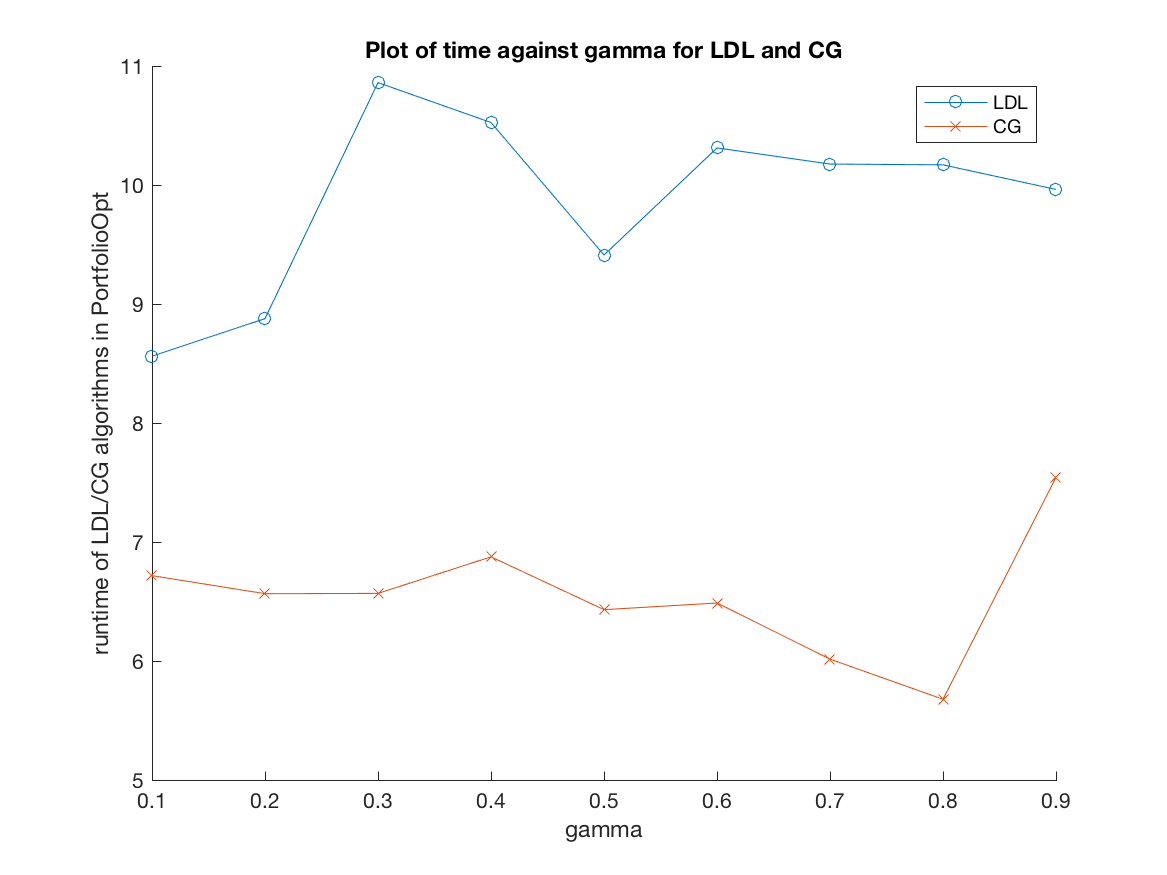
\includegraphics[width=\linewidth]{CGvsLDL_time}
	  \caption{Plot of convergence time of CG vs $LDL^T$}
	  \label{fig:cgldlt}
	\end{figure}
\end{center}

\begin{center}
	\begin{figure}[h!]
	  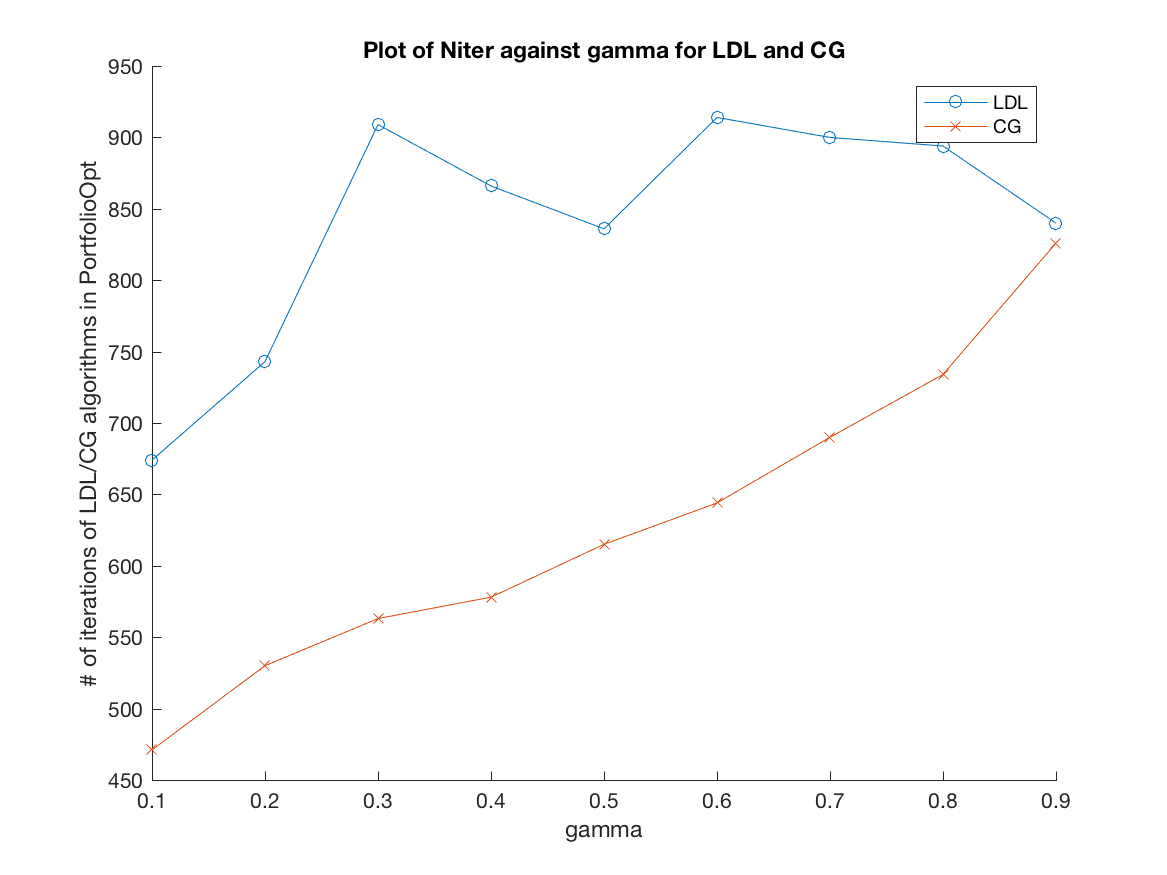
\includegraphics[width=\linewidth]{CGvsLDL_Niter}
	  \caption{Plot of iteration count of CG vs $LDL^T$}
	  \label{fig:cgldlN}
	\end{figure}
\end{center}

In general, the CG method seems to need fewer iterations but takes longer to converge than the $LDL^T$ method. The CG seems to perform worse, the closer $\gamma$ gets to 1. Iteration count increases monotonically, perhaps indicating poor conditioning increasing as $\gamma$ increases.  \\

\subsection{Four}
On inspection, $\tilde{M}$ has its largest values on the diagonal although it's certainly not diagonally dominant. Simply taking $C$ to be the values of $\tilde{M}$ on a band of width 3 about the main diagonal and zeros everywhere else would make solving the preconditioned system cost $O(N)$  and it captures a lot of the 'essence' of $\tilde{M}$ while remaining sparse.\\ 
\indent \texttt{preconCG} implements the preconditioned CG method for the aforementioned preconditioner. \texttt{qu4} runs the portfolio for varying $\gamma$ for the CG and preconditioned CG methods and captures the number of iterations and run-time of each method until convergence. These results are displayed in fig \ref{fig:cgldlN} and fig \ref{fig:cgcspre_t} respectively. 

\begin{center}
	\begin{figure}[h!]
	  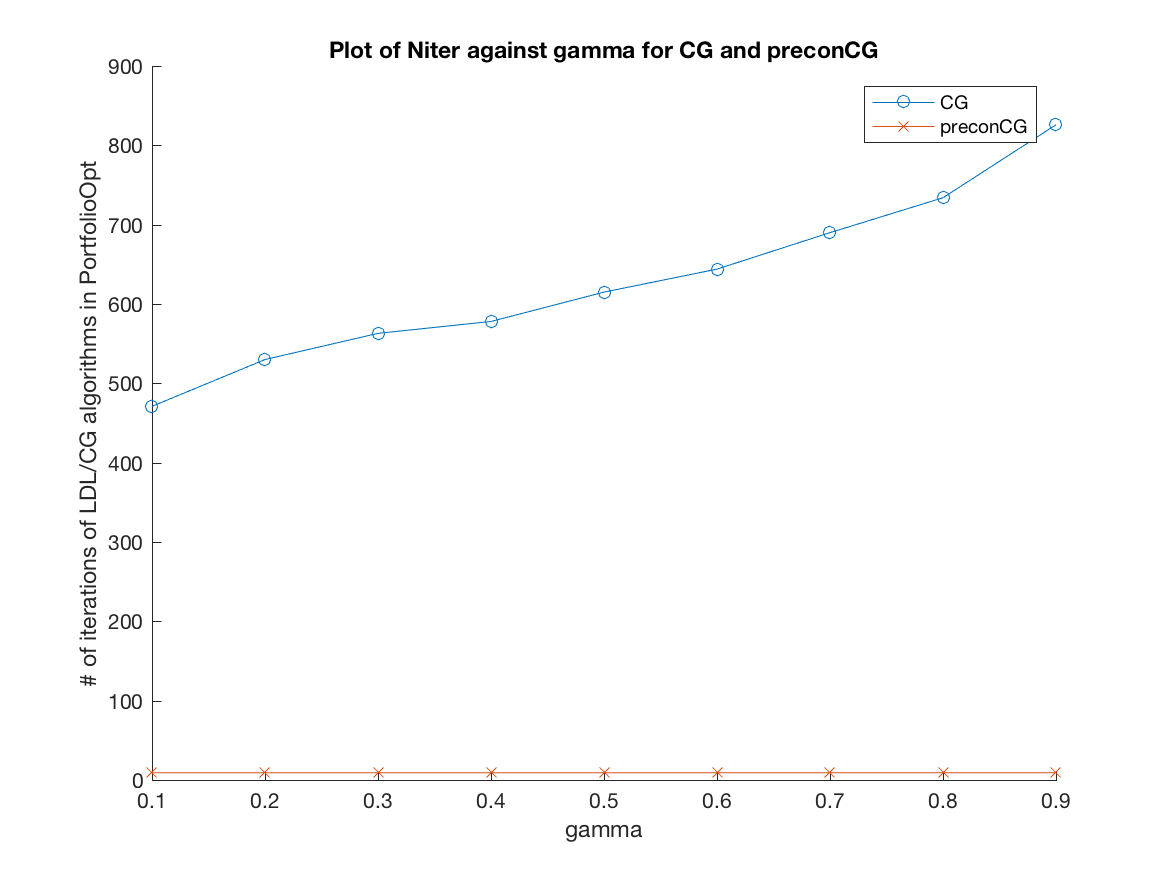
\includegraphics[width=\linewidth]{CGvspreconCG_Niter}
	  \caption{Plot of iteration count of CG vs preconditioned CG}
	  \label{fig:cgvspre_N}
	\end{figure}
\end{center}

\begin{center}
	\begin{figure}[h!]
	  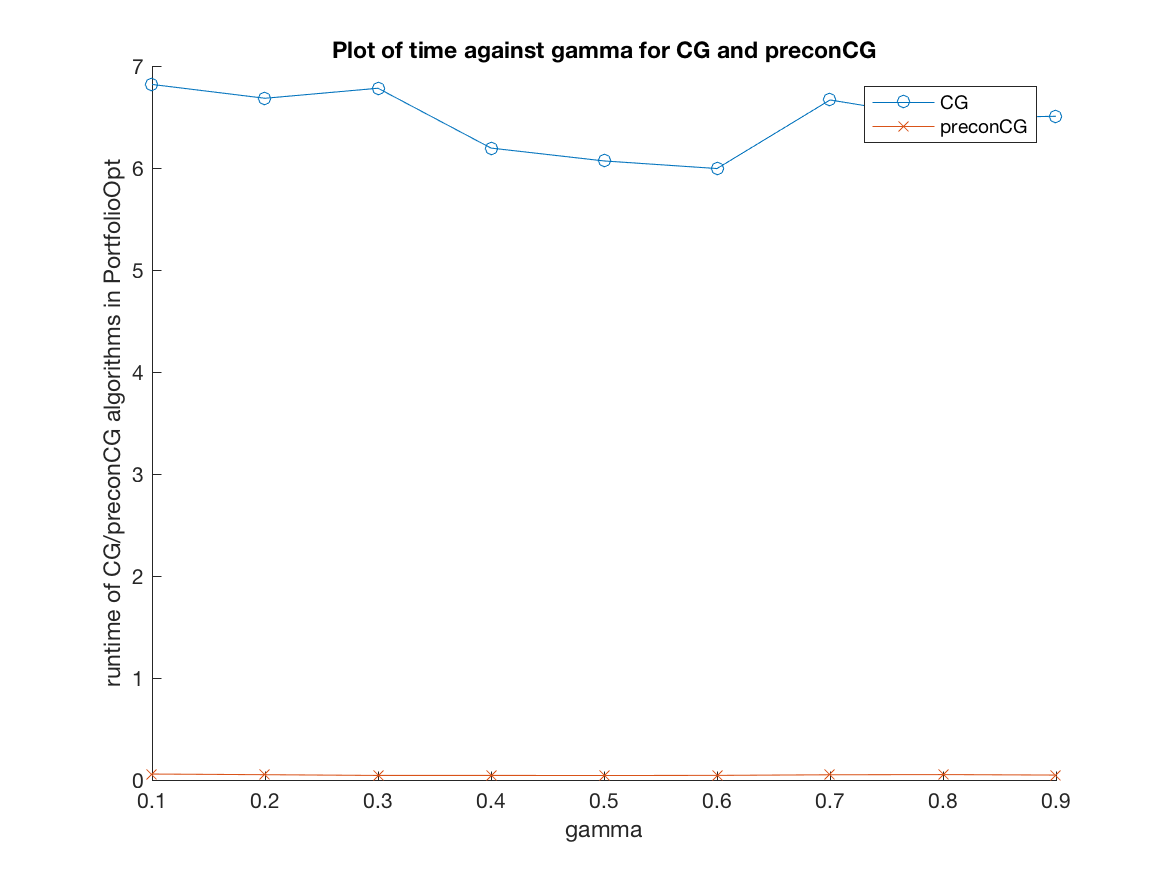
\includegraphics[width=\linewidth]{CGvspreconCG_time}
	  \caption{Plot of convergence time of CG vs preconditioned CG}
	  \label{fig:cgcspre_t}
	\end{figure}
\end{center}

We see that in fact the non-preconditioned system is blown out of the water by the speed up in convergence achieved by preconditioned system. For extra clarity, the results of the preconditioned method are in table \ref{table:4}.

\begin{table}
	\begin{center}
		\begin{tabular}{c|c}
N_preconCG = & t_preconCG = \\
\hline

     9		&    0.0574\\
     9		&    0.0509\\
     9		&    0.0436\\
     9		&    0.0439\\
     9		&    0.0429\\
     9		&    0.0442\\
     9		&    0.0502\\
     9		&    0.0521\\
     9		&    0.0473
		\end{tabular}
	\end{center}
	\caption{results from preconditioned CG}
	\label{table:4}
\end{table}
We see that N-iter and run-time are levelled out accross $\gamma$, so not only has there been a sensational speed up, but also the method is much more stable than the orignal method. 

\newpage

\section{Mastery}

\subsection{One}

The aim of the pair is to use the Lanczos process as a means to approximate $A^{\frac{1}{2}}z$, for any vector z who's entries are sampled from a normal distribution. This is motivated by the inefficient ($O(N^3)$)
method of computing a cholesky decomposition $A = SS^T$ to compute $y = A^{\frac{1}/{2}} z$ the random sample.  Preconditioning via polynomial methods are faster than factoring methods and more general than spectral methods which require highly structured (e.g block Toeplitz) matrices.

The implementation of this is as follows: let $p(A)$ be a polynomial approximating the principal square root of $A$, $A^{\frac{1}{2}}$. Generate the $m^{th}$ (say) Krylov space $K_m(A,z)$ via the Lanczos process.
  Thihe optimal approximation of $p(A)$ ts in Km is exactly its projection into $K_m$, $y_m = V_mV^T_m p(A)z$. By taking $v1 = z/\norm{z}^2$, $\beta = \norm{z}^2$ and allowing the
  approximation $V^T_m p(A) V_m \approx f(V^T_m A V_m)$, we reach the $m^{th}$ approximation $\tilde{y}_m = \beta V_m p(T_m)e_1 \approx y^{\star}$ and $p(T_m)$ is computed by some non intensive (as the number of
  iterations is low) method.\\

\indent to make convergence superlinear and more accurate, they implement preconditioning. They use the factorized sparse approximate inverse (\texttt{FSAI}) method to find such a preconditioner. This means picking a sparse lower triangular matrix G, such that $G^T G \approx A^{-1}$ motivated by and approximated to the Cholesky factor of $A^{-1}$. Which is computed on minimising the Frobenius norm 
$\norm{I - GL}_F^2 = tr((I-GL)(I-GL)^T)$
  where $L$ is the Cholesky factor of $A^{-1}$. Sparsity and lower triangularity constraints on $G$ means that it can be found inexpensively without knowing $L$.\\

Now follow the results: 
\\
\noindent The relative norm error closely matches the exact error norm in the preconditioned case for a small number of iterations before potentially spiralling off. If convergence is fast, then the estimated error is shown in examples to be more accurate than the non-preconditioned case. The upside about this is that given the ability of the preconditioner to cluster the spectrum of $T_m$ around one eigenvalue and convergence is expected to be much faster than other linear methods and so the estimation of the absolute error can be said to be accurate.\\ 

\noindent For sparse matrices, $A$ more iterations risks loss of orthogonality between the basis vectors. Reorthogonalization can be done but is not standard and inevitably adds
computation to the problem. In cases where the matrix is ill-conditioned (e.g piecewise polynomial covariance matrices with higher l value) more iterations are required by the algorithm for the untreated matrix which leads to greater risk of losing orthogonality. As the preconditioned matrix reduces the condition number
and converges in fewer iterations (as well as with lower run-time) there is lower risk of losing orthogonality. So for potentially ill-conditioned matrices, the benefit is large.
Also for sparse matrices, the Cholesky factor method was shown to be much slower than the polynomial approximation method. The results again show that preconditioning reduces the iteration count and computation time for computing a sample vector.\\

\noindent For dense matrices, $A$ the paper showed a dramatic decrease in number of iterations and computation time, particularly as the size of the matrix increases. The effect of \texttt{FSAI} actually greater
here than for sparse matrices. The time taken to precondition is minimal even in very large cases. In larger cases 'set up' time is vastly outweighed by the iteration time. In smaller cases it can be around the same order as the iteration time, but even in sum this is much less than the computation time in the unpreconditioned case.
Again, Cholesky factorisation was shown to take an extremely long time in the largest case.

An interesting parting note was that stencil size (how many non-zero elements per column in G) has an optimal value. If the stencil size is increased too greatly then set up time becomes large and iteration time is not decreased which is negative.

\subsection{Two}
The script \texttt{qu2} generates a pseudo random vector of length 10, creates M for b=3, n=5 then computes the $V_m$ and $T_m$ for successive m via the function \texttt{lanczos}. It then proceeds to find the principal root of T via \texttt{pRoot}. \texttt{pRoot} computes the eigenvalues of T via \texttt{wilkinsonQR}, creates a diagonal matrix, D of the sqrt of the eigenvalues, uses \texttt{invItr} to find the an orthogonal matrix of eigenvectors and computes $T{\frac{1}{2}} = Q D^{\frac{1}{2}} Q^T$. \\
invItr has been since part 2. Now it uses the fact that T is spd to implement a quicker solver. It now uses the Thomas algorithm in \texttt{spdTriSolver} which, while still $O(N)$ is still quicker than non-symmetric tridiagonal solver \cite{3}. \\ 

Running \texttt{qu2} spits out 

\begin{table}
	\begin{center}
		\begin{tabular}{c}

			y = \\
			\hline
			    0.2201\\
			    0.0366\\
			    0.2097\\
			    0.1863\\
			    0.1705\\
			    0.0969\\
			    0.1009\\
			    0.1903\\
			    0.0756\\
			    0.0519\\
					
		\end{tabular}
	\end{center}
	\caption{y for b=3, n=5 as solved by the unpreconditioned method in Chow \& Saad}
	\label{table:3}
\end{table}

\subsection{Three}
The example process above is generalized into a function, \texttt{A12z}, which takes and $b, n$ and random vector $z$ to give the approximation of $A^{\frac{[1]}{2}}$. The script \texttt{qu3} runs \texttt{A12z} for $b \in 3:12$ and $N \in 100:30:600$ and creates two $10\times 10$ matrices for run-time and N-iter over the values for $b, N$. It Uses these matrices to plot contour plots \ref{fig:mas1} and \ref{fig:mas2}. 

\begin{center}
	\begin{figure}[h!]
	  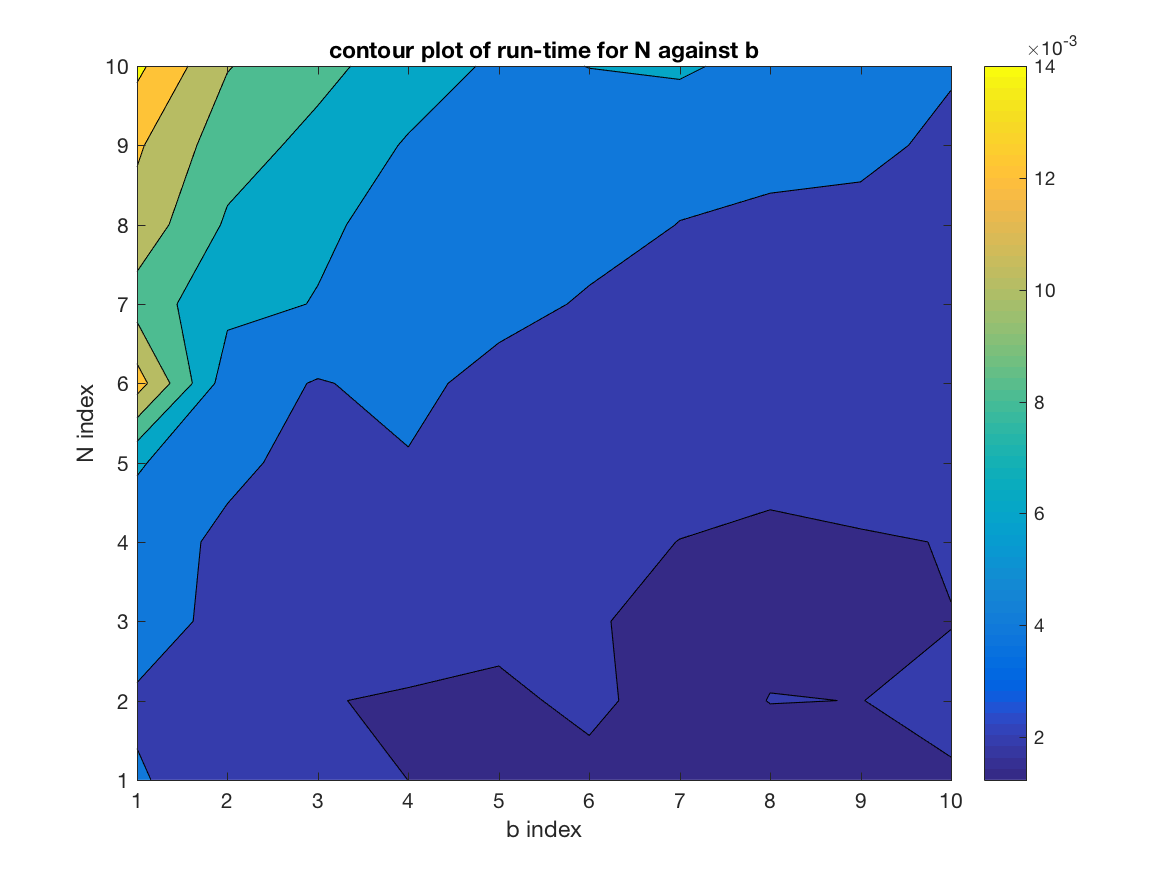
\includegraphics[width=\linewidth]{mastq4time}
	  \caption{Plot of b against N contoured by run-time }
	  \label{fig:mas1}
	\end{figure}
\end{center}

\begin{center}
	\begin{figure}[h!]
	  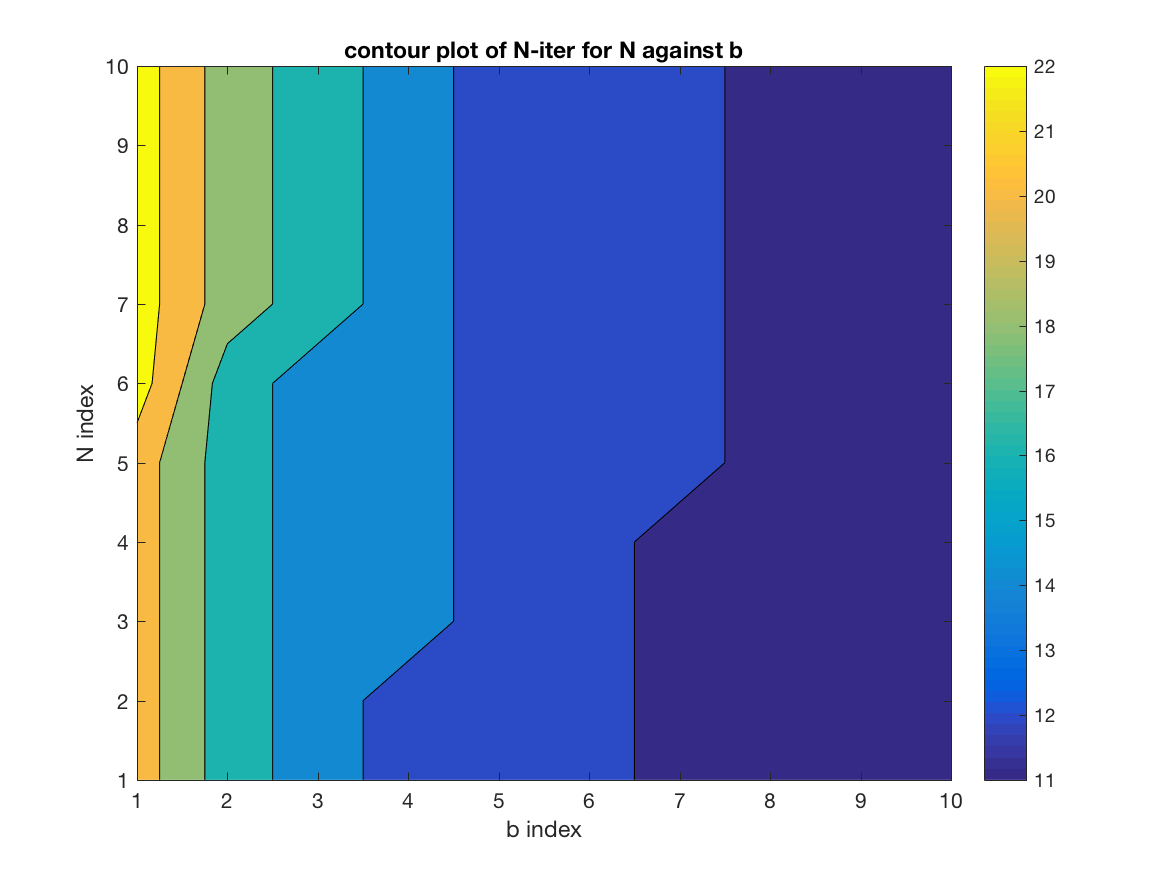
\includegraphics[width=\linewidth]{mastq4iter}
	  \caption{Plot of b against N contoured by N-iterations}
	  \label{fig:mas2}
	\end{figure}
\end{center}

The figures show that for high values of N and low values of b, the number of iterations and run-time increase. For the values considered, the number of iterations is not too high. \\
As b stays low and N increases conditioning may become necessary. I would recommend using a FSAI preconditioner as the structure of the matrices has a static structure which makes this a good choice. 

\newpage

\addcontentsline{toc}{section}{Appendix}
\newpage
\begin{appendix}
\listoffigures
\listoftables

\end{appendix}
\addcontentsline{toc}{section}{References}
\begin{thebibliography}{3}
 \bibitem{1}
 Tridiagonalization of a Symmetric Band Matrix, Schwarz, H. R. 1971 \\
	DOI 10.1007/978-3-662-39778-7\_19, pages 273–283\\
 
 \bibitem{2}
	A Wilkinson-like multishift QR algorithm for symmetric eigenvalue problems and its global convergence. \\ (2011, April 17). Retrieved January 12, 2018, from \\  \texttt{https://www.sciencedirect.com/science/article/pii/S0377042711001890}
\bibitem{3}
Golub, G. H., \& Loan, C. F. van. (2013). Matrix computations. Baltimore: Johns Hopkins University Press.

\end{thebibliography}

\end{document}







